\documentclass[a4paper,titlepage,10pt]{article}

\usepackage[T1]{fontenc}
\usepackage[utf8]{inputenc}
\usepackage{polski}

\usepackage{enumerate}
\usepackage{amssymb}
\usepackage{amsmath}
\usepackage[pdftex]{graphicx}
\usepackage{tikz}
\usepackage[colorlinks=true,linkcolor=blue]{hyperref}
\usepackage{anysize}

\usepackage{lastpage}
\usepackage{fancyhdr}

\usepackage{pdflscape}

\usepackage[a4paper, top=2.5cm, bottom=2.5cm, left=2cm, right=2cm]{geometry}
\linespread{1.3}

\title{\huge Symulacja układu planetarnego na GPU\\ przy użyciu CUDA i OpenGL\\\small Dokumentacja techniczna}
\author{Daniel Kłobuszewski\and Jakub Kotur}

\begin{document}
	\maketitle
	
	\pagestyle{fancyplain}
%        \fancyhf{}
	\cfoot{\thepage/\pageref{LastPage}}

	\hfill \\
	\begin{figure}[h]
	\centering
\begin{tabular}{|p{.1\textwidth}|p{.04\textwidth}|p{.1\textwidth}|p{.1\textwidth}|p{.206\textwidth}|p{.1\textwidth}|}
	\hline
	\multicolumn{6}{|l|}{Metryka dokumentu} \\
	\hline
	Projekt & \multicolumn{2}{l|}{Symulacja układu planetarnego na GPU } &
	Firma & \multicolumn{2}{l|}{Politechnika Warszawska} \\
	&  \multicolumn{2}{l|}{przy użyciu CUDA i OpenGL} & &  \multicolumn{2}{l|}{} \\
	\hline
	Nazwa & \multicolumn{5}{l|}{Dokumentacja techniczna} \\
	\hline
	Temat & \multicolumn{5}{l|}{Specyfikacja techniczna projektu} \\
	\hline
	Autor & \multicolumn{5}{l|}{Daniel Kłobuszewski, Jakub Kotur} \\
	\hline
	Plik & \multicolumn{5}{l|}{tech.pdf} \\
	\hline
	Nr wersji & 06 & Status & Finalny & Data\par sporządzenia & 2010-10-09 \\
	\hline
	Streszczenie & \multicolumn{5}{p{11cm}|}{Celem dokumentu jest zdefiniowanie
		technicznych wymagań Projektu.} \\
	\hline
	Zatwierdził & \multicolumn{3}{l|}{ } &
	Data ostatniej\par modyfikacji & 2010-10-12 \\
	\hline
\end{tabular}

	\label{tab:metric}
\end{figure}


	\hfill \\
	%\newpage
	\begin{figure}[h]
	\centering

\begin{tabular}{|p{.075\textwidth}|p{.1\textwidth}|p{.2\textwidth}|p{.522\textwidth}|}
	\hline
	\multicolumn{4}{|l|}{Historia zmian dokumentu} \\
	\hline
	Wersja & Data & Kto & Opis \\
	\hline
	0.1 & 2011-01-02 & Jakub Kotur &
	Określenie podstawowej struktury dokumentu \\
	\hline
	0.2 & 2011-01-04 & Jakub Kotur &
	Dodanie opisów dziłania oraz zmian \\
	\hline
	1.0 & 2011-01-04 & Daniel Kłobuszewski &
	Poprawki ortograficzne i stylistyczne \\
	\hline
\end{tabular}

	\label{tab:hist}
\end{figure}



	\newpage

	\tableofcontents
	\newpage

	\section{Streszczenie}\label{sec:streszczenie}
	\paragraph{}
Poniższy dokument stanowi podsumowanie projektu, pisanego w ramach przedmiotu Projekt Zespołowy, na wydziale Matematyki i Nauk Informacyjnych Politechniki Warszawskiej w semestrze zimowym 2010/2011.

\paragraph{}
Opisujemy w nim zasady działania głównych modułów, różnice w stosunku do specyfikacji oraz wnioski z testów akceptacyjnych. Znajduje się tutaj także krótka instrukcja obsługi programu, która pozwoli zapoznać się z nim każdej osobie, która wcześniej nie miała z naszą aplikacją styczności.

	\section{Uzyte technologie}\label{sec:uzyte technologie}
	\paragraph{}

Jednym z podstawowych założeń tego projektu jest użycie technologii CUDA. Daje to nam możliwość oprogramowania karty graficznej, ale stawia też ograniczenia. Przede wszystkim jesteśmy zmuszeni używać języka C (konkretniej, C for CUDA) do części uruchamianej na procesorze graficznym. Najłatwiej używać go wspólnie z C++ na CPU. Oczywiście istnieją bindingi w innych językach (Java, Python), ale C++ jest z nich najszybszy - nie uwzględniając czystego C, które jednak nie wspiera obiektowości. 

\paragraph{}

Kod pisany na kartę graficzną nie będzie napisany w języku obiektowym, więc wszystkie klasy, które zdefiniowaliśmy dla jednostki graficznej są jedynie abstrakcją, która pośrednio się na niego przekłada. Chcemy uzyskać aplikację wydajnie korzystającą z karty graficznej, w związku z czym ułożenie "obiektów" w pamięci będzie pozwalało na szybki i wygodny dostęp do nich. Prawdopodobnie w pewnych miejsacach spowoduje to zmniejszenie czytelności kodu na rzecz prędkości jego wykonania.

	\section{Architektura projektu}\label{sec:architektura projektu}
	\subsection{Działanie programu}\label{sub:dzialanie programu}
	\paragraph{}

Podstawowymi aktywnościami projektu są moduły wyświetlania planet oraz obliczania pozycji planet. Jednak dla działania aplikacji bardzo ważne są również inne aktywności, które mimo, że prostsze w implementacji mają duży wpływ na architekturę projektu. Poniższy diagram przedstawia kolejne aktywności aplikacji podczas działania. Dodatkowo przedstawiony na diagramie jest przepływ najważniejszych informacji, czyli pozycji planet.

\paragraph{}

\begin{figure}[ht!]
	\centering
	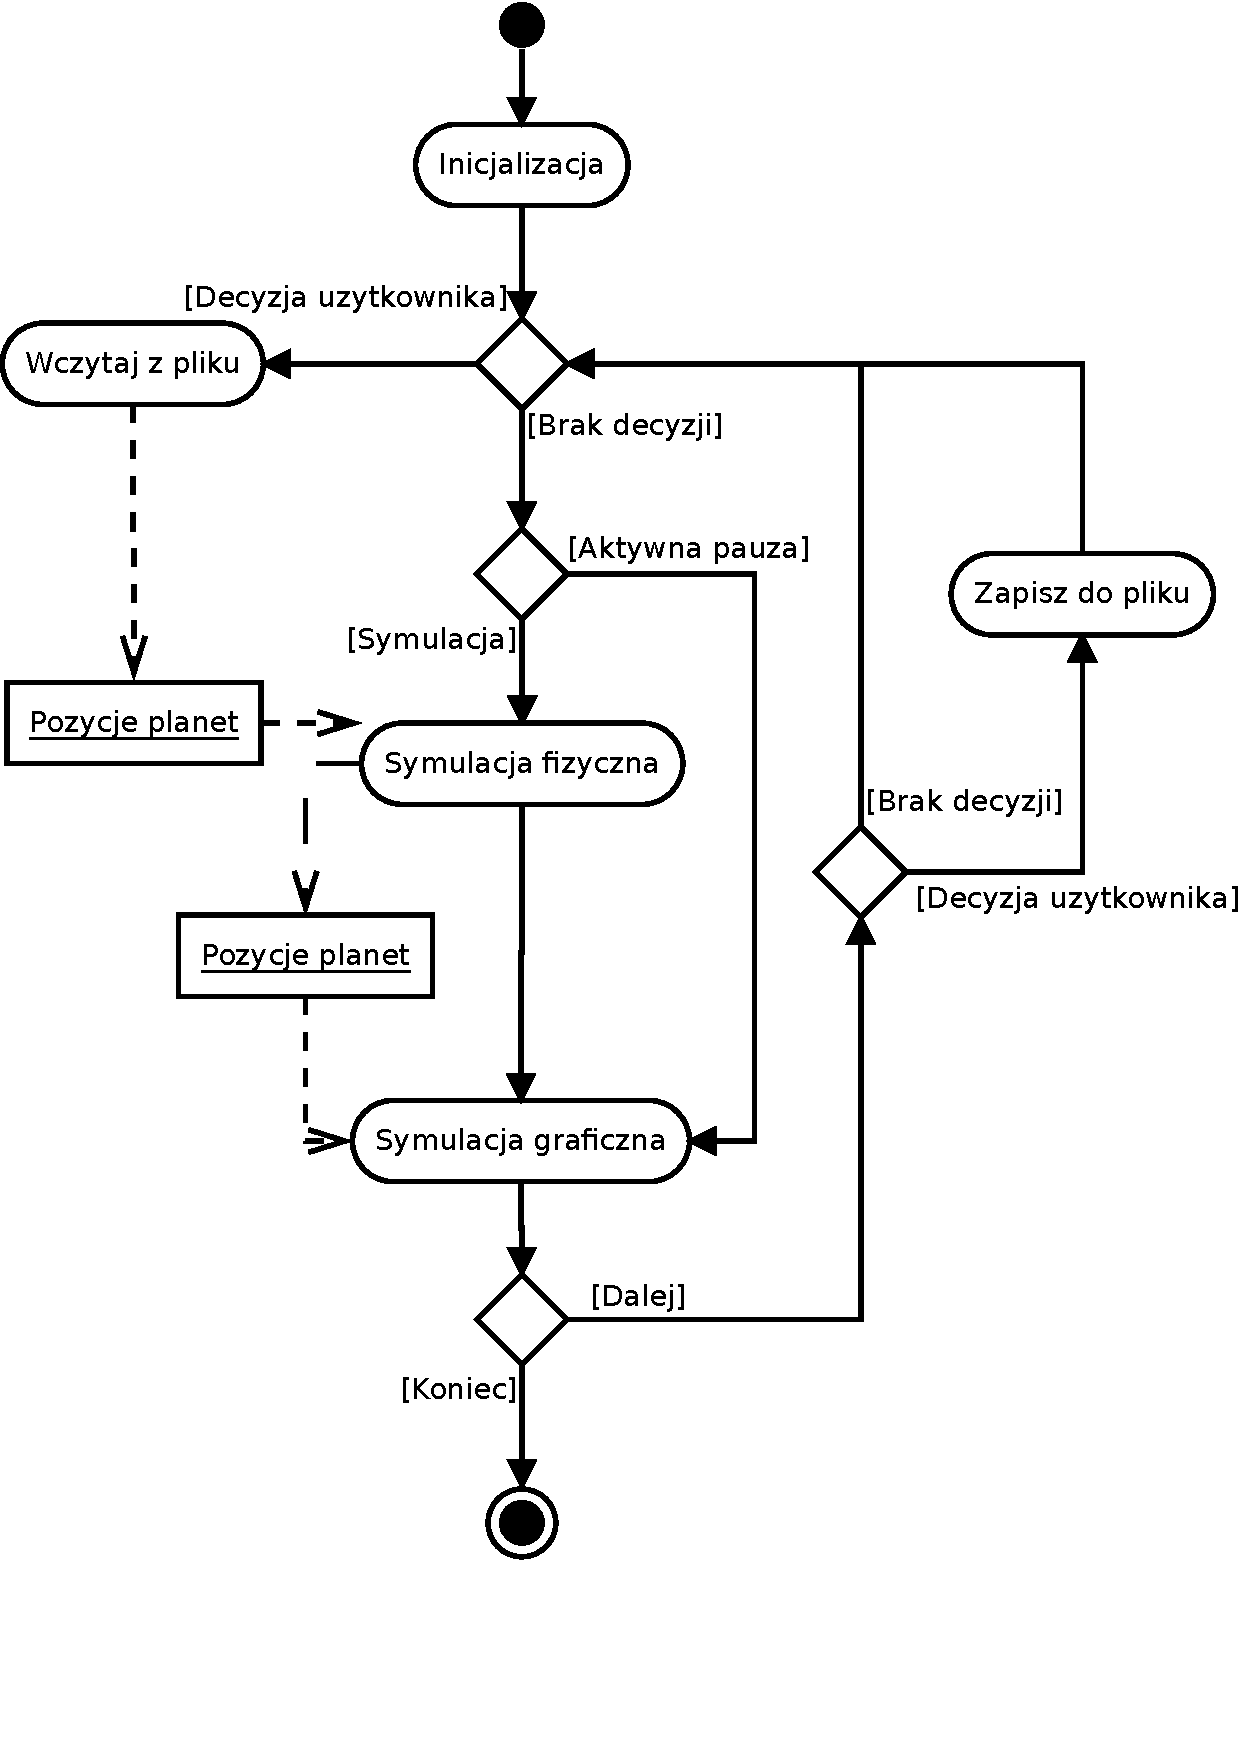
\includegraphics[width=0.75\textwidth]{activity.pdf}
	\caption{Diagram aktywności}
	\label{fig:activity}
\end{figure}


\begin{description}
	\item[Inicjalizacja aplikacji] \hfill \\
	Jest to pierwsza aktywność jaką wykonuje program. Składa się ona z inicjalizacji wszystkich modułów, w szczególności modułu graficznego i fizycznego. Zajmuje się także początkową alokacją pamięci i wczytaniem wszystkich potrzebnych zasobów, takich jak tekstury, modele oraz inne potrzebne dane.
	\item[Wczytanie z pliku] \hfill \\
	Jeśli użytkownik zdecyduje zacząć symulację z wcześniej przygotowanego pliku ta akcja jest za to odpowiedzialna. Musi ona załadować potrzebne dane z pliku oraz zapisać je poprzez pamięć RAM jednostki głównej do pamięci RAM jednostki graficznej. Użytkownik może również zdecydować o wczytaniu z pliku podczas już trwającej symulacji. W takim przypadku konieczne jest również zadbanie o odpowiednie wyczyszczenie poprzedniej symulacji, tak aby żadne artefakty nie zostały w pamięci RAM jednostki głównej ani graficznej.
	\item[Zapis do pliku] \hfill \\
	Na życzenie użytkownika aktualny stan symulacji może zostać zapisany do pliku. W takim przypadku zbierane z aplikacji są wszystkie potrzebne dane, takie jak pozycje planet, wielkości i ciężary planet, modele planet, pozycja kamery itp., oraz zapisywane są do pliku.
	\item[Aktywna pauza] \hfill \\
	Symulacja wspiera tak zwaną "aktywną pauzę". Oznacza to, że na żądanie użytkownika symulacja fizyczna jest zatrzymana, natomiast cały czas reszta aplikacji jest w pełni funkcjonalna. Oznacza to, że można sterować kamerą, wczytywać/zapisywać układy planetarne oraz dodawać/usuwać planety.
	\item[Symulacja fizyczna] \hfill \\
	Jest to kluczowy moduł dla działania aplikacji. Podczas każdej takiej aktywności obliczane są kolejne pozycje planet do wyświetlenia. W jednej takiej akcji może być obliczona więcej niż jedna klatka fizyczna, jeśli moc obliczeniowa komputera na to pozwala.
	\item[Symulacja graficzna] \hfill \\
	Ta aktywność odpowiedzialna jest przede wszytkim za wyświetlanie symulacji na ekranie. Głównym jej zadaniem jest wyświetlanie planet na ich pozycjach wraz z towarzyszącymi im efektami graficznymi. Pozycje planet do wyświetlenia pobierane są z modułu fizycznego. Jeśli natomiast jest włączona aktywna pauza i nowe pozycje nie zostały wygenerowane, moduł korzysta ze starych pozycji. Po zakończonej jednej iteracji pętli, aplikacja odczekuje chwilę, żeby nie zajmować całego procesora oraz żeby zapewnić takie samo działanie symulacji na słabszych komputerach (gdzie czekanie może zostać pominięte)
\end{description}


	\subsection{Struktura klas}\label{sub:struktura klas}
	\paragraph{}
Ze względu na architekturę aplikacji, klasy używane na CPU oddzielone są od klas karty graficznej. Oczywiście te drugie są klasami jedynie logicznie - ze względu na konieczność używania języka C w kodzie dla GPU. Ponieważ jednak obiekty są wygodną abstrakcją, będziemy z niej korzystać w całym programie.

\subsubsection{Klasy GPU}

\begin{figure}[h]
	\centering
	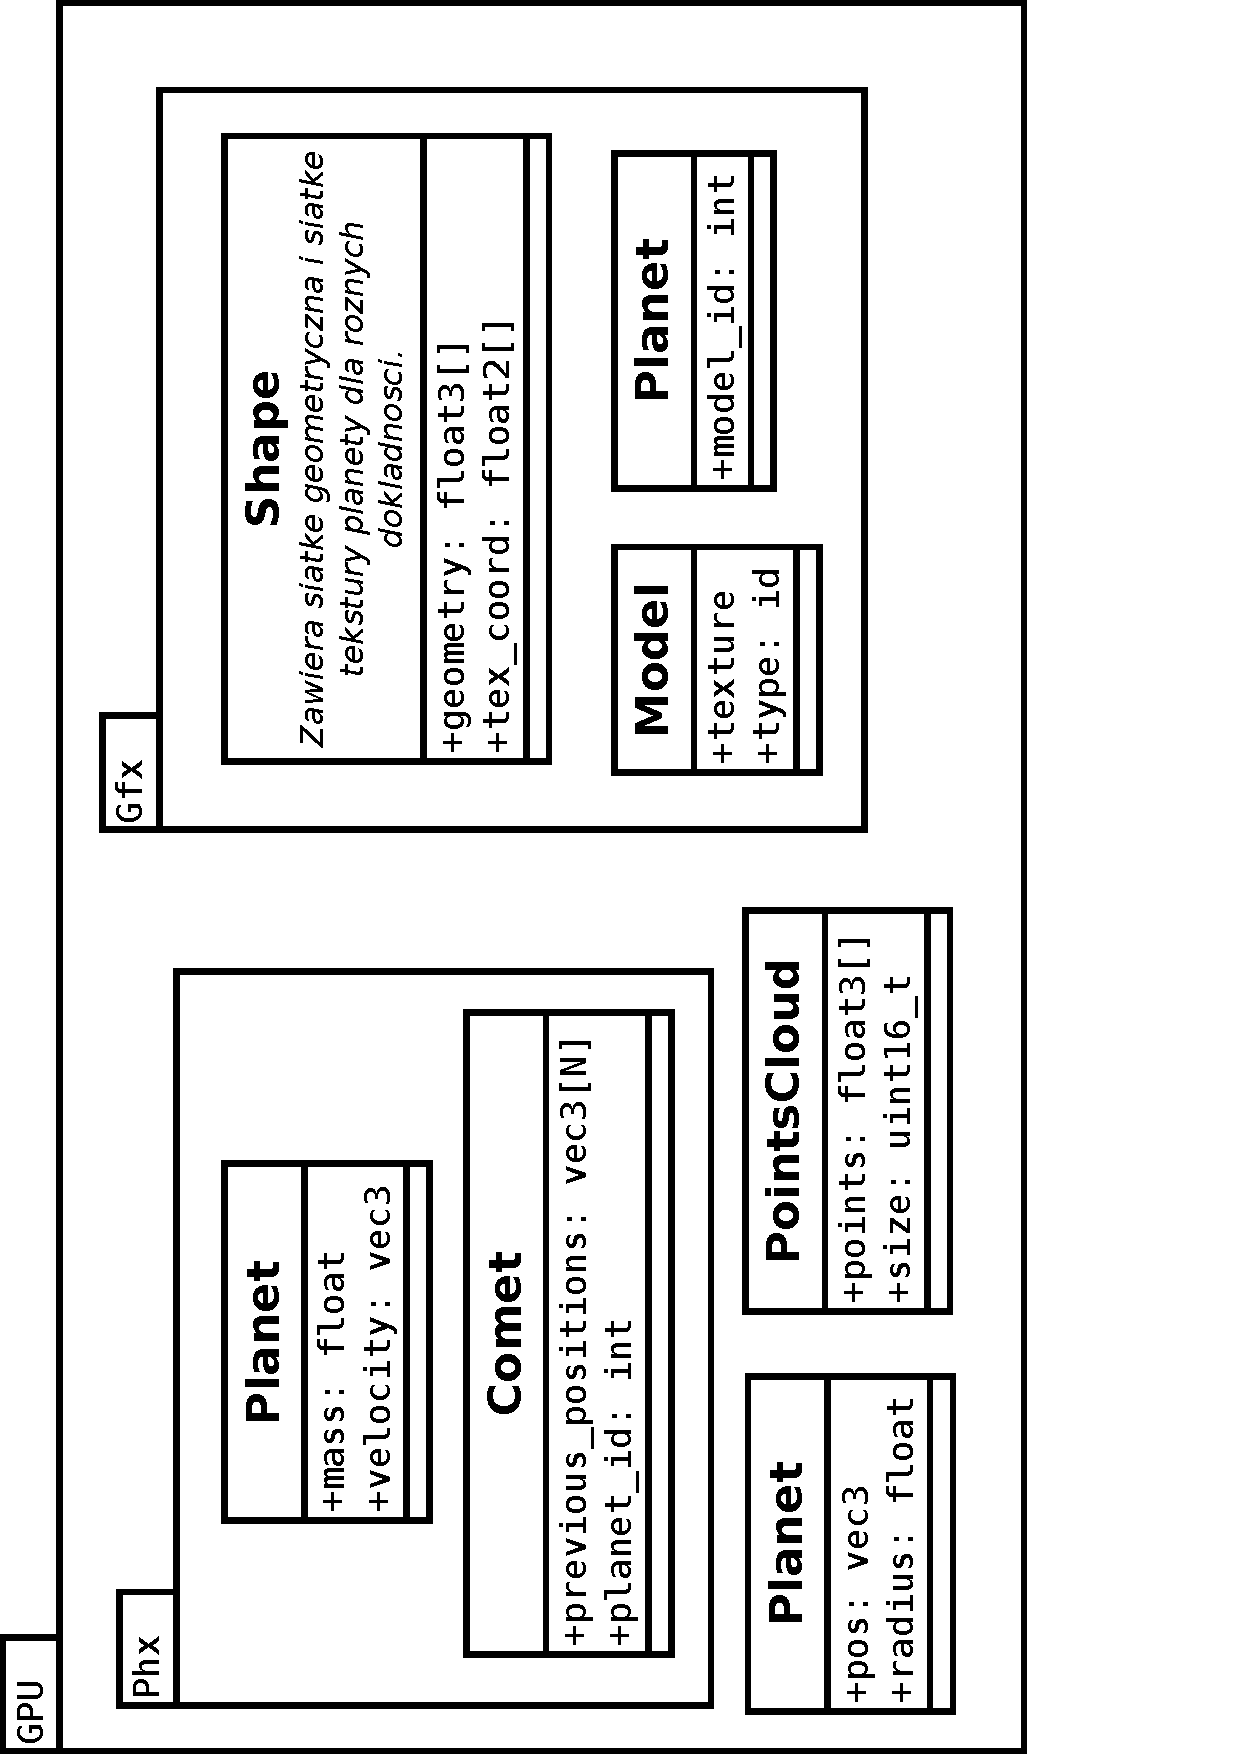
\includegraphics[angle=270,width=0.8\textwidth]{class_gpu.pdf}
	\caption{Diagram klas dla GPU}
	\label{fig:class_gpu}
\end{figure}

\paragraph{}
Struktury, z których będziemy korzystać na karcie graficznej, określone są na rysunku \ref{fig:class_gpu}. Ponieważ karta graficzna służy nam zarówno do wyświetlania danych, jak i do ich przetwarzania, wydzielone są na nim dwie przestrzenie nazw. Są to:
\begin{itemize}
	\item{Phx - do operacji fizycznych}
	\item{Gfx - do operacji graficznych}
\end{itemize}

\paragraph{}
Ponadto istnieje kilka struktur wspólnych dla obu częsci.

\paragraph{GPU::Planet} zawiera informacje, z których korzystaja zarówno wyświetlanie jak i fizyka. Jest to położenie planety oraz jej promień.
\paragraph{GPU::PointsCloud} reprezentuje chmurę cząstek - jest ona obliczana dla każdej widocznej komety przez moduł fizyczny.

\paragraph{}
Operacje fizyczne odbywać się będą z wykorzystaniem dwóch dodatkowych struktur.

\paragraph{GPU::Phx::Planet} to dodatkowe informacje o każdej planecie, które są potrzebne jedynie silnikowi fizycznemu. Należą do nich prędkość oraz masa.
\paragraph{GPU::Phx::Comet} stanowi dodatkową informację o planecie. Struktura ta istnieje tylko dla obiektów będących kometami. Zawiera kilka ostatnich pozycji oraz identyfikator planety.

\paragraph{}
Do wyświetlenia planet konieczne będą informacje o teksturach, oraz o siatkach każdej z planet.

\paragraph{GPU::Gfx::Planet} zawiera indeks modelu, czyli wyglądu planetu. Dwie planety mogą mieć ten sam model.
\paragraph{GPU::Gfx::Model} definiuje konkretny wygląd. Na tym poziomie będziemy rozróżniać zwykłe planety od gwiazd i komet.
\paragraph{GPU::Gfx::Shape} agreguje informację o siatce planety w 3D oraz odpowiadającej jej siatce na dwuwymiarowej teksturze.

\subsubsection{Klasy CPU}

\begin{figure}[h]
	\centering
	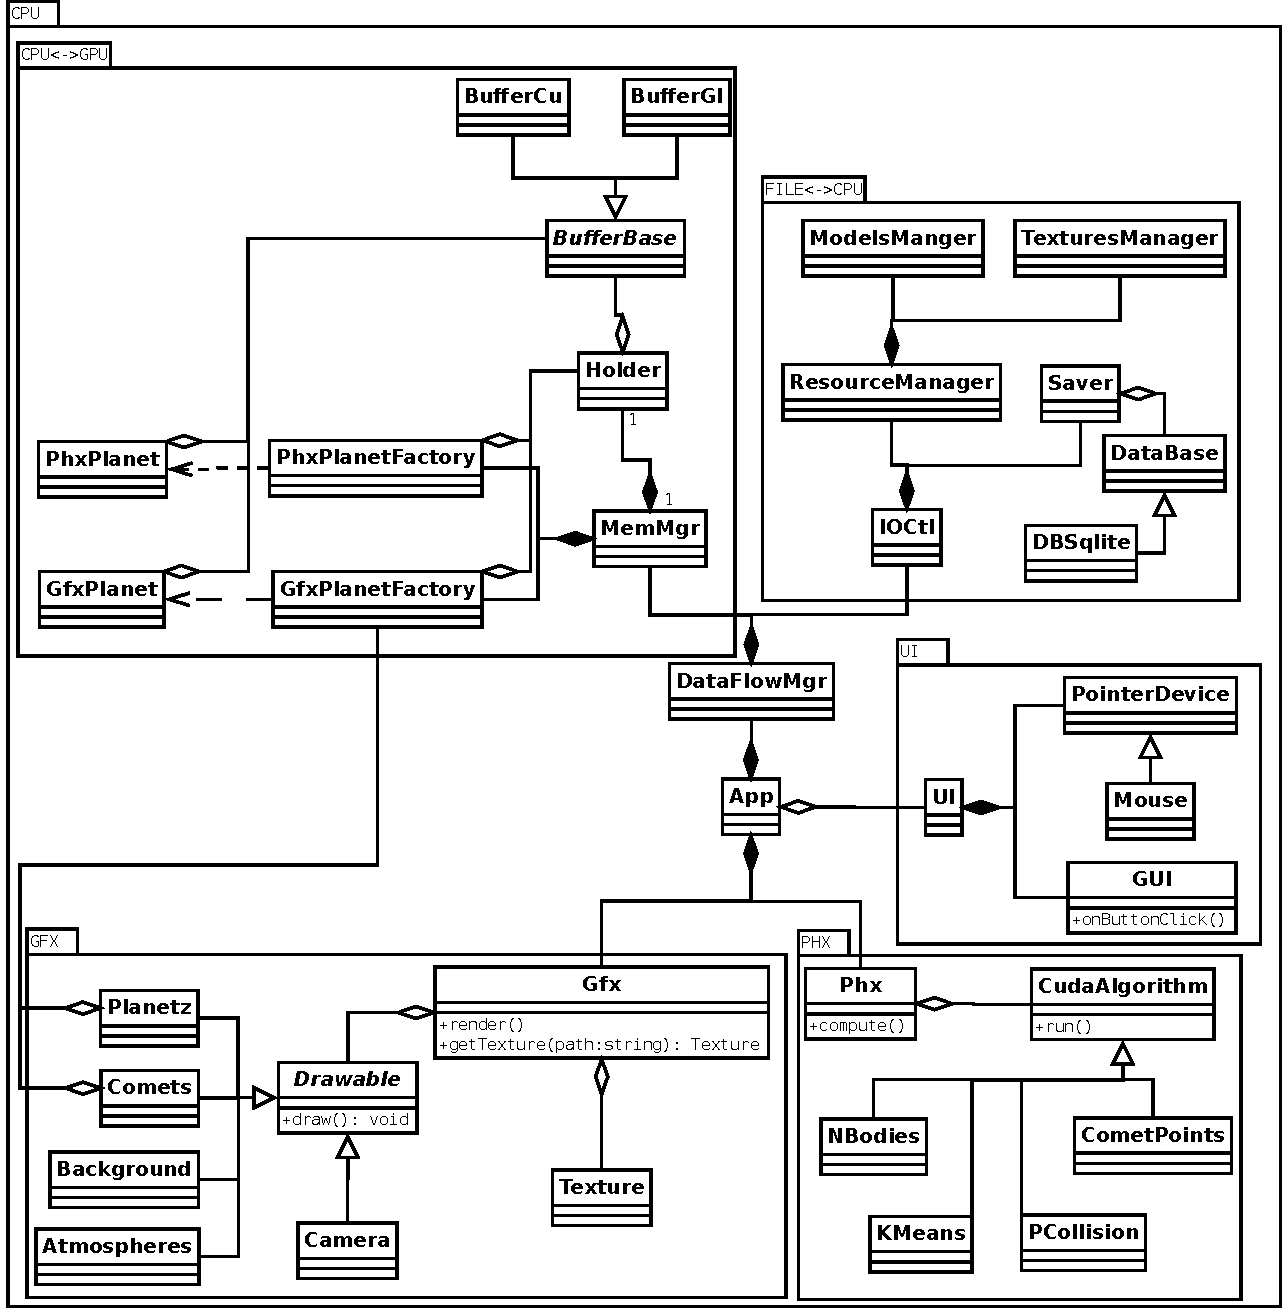
\includegraphics[angle=270,width=0.8\textwidth]{class_cpu.pdf}
	\caption{Diagram klas dla CPU}
	\label{fig:class_cpu}
\end{figure}

\paragraph{}
Ta część klas przełoży się bezpośrednio na klasy znane z c++. Diagram klas znajduje się na rysunku \ref{fig:class_cpu}.

\paragraph{CPU::App} jest główną klasą, zarządzającą obiektami GFX, PHX, DataFlowMgr oraz UI. Tworzy je ona na początku działania programu.
\paragraph{CPU::GFX} odpowiada za wyświetlanie. Korzysta przy tym z biblioteki OpenGL.
\paragraph{CPU::PHX} uruchamia kernel'e CUDA, które przeprowadzają wszystkie obliczenia fizyczne.
\paragraph{CPU::DataFlowMgr} wykonuje wszystkie przepływy danych - pomiędzy RAM karty graficznej, RAM komputera oraz dyskiem twardym.
\paragraph{CPU::MemMgr} na zlecenie DataFlowMgr'a przenosi dane pomiędzy kartą graficzną a RAM.
\paragraph{CPU::IOCtl} na zlecenie DataFlowMgr'a przenosi dane pomiędzy RAM a dyskiem twardym.
\paragraph{CPU::UI} odpowiada za całość interakcji z użytkownikiem.
\paragraph{CPU::GUI}, czyli graficzny interfejs użytkownika. Obsługa okienek.
\paragraph{CPU::InputDev} obsługuje klawiaturę i mysz.
\paragraph{CPU::PlanetPicker} służy do określania, która planeta została zaznaczona.

	\section{Implementowane algorytmy}\label{sec:implementowane algorytmy}
	\subsection{Efekty graficzne}\label{sub:algorytmy graficzne}
	\subsection{Oświetlenie}\label{sub:oswietlenie}

\paragraph{}

Oświetlenie dla sceny będzie liczone przy pomocy model Phonga. Polega to na policzeniu oświetlenia dla trzech różnych rodzai światła, oraz dodaniu ich, korzystając z prawa addytywności światła. Pierwszym z nich jest światło rozproszone, obecne na całej w takim samym natężeniu. Drugim światłem jest światło . Ten rodzaj światła uwzględnia położenie oświetlenia względem powierzchni. Pozwala to na uzyskanie realistycznych matowych powierzchni. Trzecim rodzajem jest światło odbite. Uwzględnia ono zarówno położenie wierzchołka względem światła, jak i pozycji obserwatora. Dzięki temu można uzyskać realistyczne efekty powierzchni gładkich i błyszczących.

\paragraph{}

W zależności od możliwości obliczeniowych, model oświetlenia może mieć kilka ograniczeń. Oświetlenie można obliczać dla każdego wierzchołka, natomiast kolor ściany interpolować liniowo pomiędzy kolorami wierzchołków na który składa się dana ściana. Można też obliczać natężenie światła dla każdego piksela z którego składa się ściana. Oczywistym jest że w drugim przypadku obliczenia są znacząco większe niż w przypadku pierwszym. Ograniczeniom podlega również ilość świateł obecnych na scenie. Dla każdego światła trzeba powtórzyć obliczenia dla wszystkich wierzchołków na scenie. Aby zachować płynność symulacji, ilość świateł, a zatem gwiazd, będzie ograniczona przez pewną stałą liczbę ustaloną na podstawie testów w fazie implementacji.

\subsection{Efekt atmosfery}\label{sub:efekt atmosfery}

Aby uzyskać efekt atmosfery otaczającej planety, można zastosować dwa odmienne podejścia. Decyzja które z nich zostanie wybrane, pozostawiona została do fazy implementacji, ponieważ zależy to mocno od wydajności całego silnika graficznego.

\paragraph{}

Efekty atmosferyczne mogą być generowane przy pomocy techniki post-processingu. Polega to na nakładaniu obrazu, na już uzyskany obraz w trakcie normalnego renderowania sceny 3D. W przypadku atmosfer, należy wygenerować lekko rozmyte okręgi w miejscach gdzie wyrenderowane zostały planety z odpowiednim promieniem.

\paragraph{}

Drugim rozwiązaniem jest otoczenie planet półprzezroczystymi sferami, o promieniu trochę większym niż promień planet. Rozwiązanie ma tą zaletę, że całym procesem wyświetlania zajmuje się biblioteka graficzna. Minusem może być wydajność, choć nie jest to konieczne.


\subsection{Dynamiczna szczegółowość planet}\label{sub:dynamiczna szczegolowosc planet}

\paragraph{}

W zależności od odległości od obserwatora, planety powinny być wyświetlane z różnym poziomem szczegółowości. Rozwiązaniem będzie wyświetlanie modelu kuli, o mniejszej ilości wierzchołków. Wszystkie modele ładowane będą na początku z pliku, do pamięci ram karty graficznej, skąd będą później wyświetlane, w zależności od tego który model będzie aktualnie potrzebny.

\subsection{Komety}\label{sub:komety}

\paragraph{}

Warkocz komety jest typowym przykładem efektu cząsteczkowego. Dla chmury wygenerowanych cząsteczek, wyświetlana jest niewielka tekstura z kamieniem, bądź ogniem. Dzięki dużej ilości takich tekstur, powstanie realistyczny obraz płomienia ciągnącego się za kometą.


	\subsection{Algorytmy fizyczne}\label{sub:algorytmy fizyczne}
	\subsubsection{Klasteryzacja}

\paragraph{}

Do pogrupowania planet w klastry użyty zostanie algorytm k-means. W algorytmie tym na zmianę znajdujemy środki klastrów, po czym przyporządkowujemy punkty do najbliższego środka. K-means bardzo dobrze nadaje się do naszych celów, biorąc pod uwagę, iż zwykle planety i tak będą zgrupowane wokół masywniejszych gwiazd. Ułatwi to i przyspieszy pracę algorytmu, gdyż zwykle wybór punktów początkowych ma kluczowy wpływ na czas działania oraz wynik. Jako początkowe środki klastrów będzie można wziąć środki k najmasywniejszych obiektów. Wyznaczenie wartości k, a zatem ilości klastrów, będzie wykonywane na podstawie ilości oraz mas klastrowanych obiektów.

Zasada działania algorytmu k-means została zapisana poniżej w pseudokodzie:

\begin{enumerate}
	\item{Wybierz k punktów przestrzeni, będą to środki klastrów}
	\item{Każdy z punktów do klasteryzacji przydziel do klastra, którego środek jest najbliższy}
	\item{Wyznacz błąd kwantyzacji: \ensuremath{D = {1\over{n}}\sum_{i = 1}^{n}d(x_i, r)}, gdzie \ensuremath{r} jest środkiem klastra, do którego należy \ensuremath{x_i} }
	\item{Jeżeli \ensuremath{\frac{\Delta{D}}{D}\geqslant\epsilon}, wyznacz nowe środki klastrów (jako średnie z punktów w tych klastrach) i przejdź do punktu 2.}
\end{enumerate}

	\section{Format zapisu danych}\label{sec:format zapisu danych}
	\paragraph{}

Pliki, z których korzysta aplikacja, będą bazami danych sqlite. Dzięki temu będziemy mogli w łatwy sposób z nich korzystać.

\paragraph{}

W bazie opisującej symulację znajdzie się kilka tabel. Najważniejsza z nich to tabela "planets". Znajdą się w niej te same pola, co w odpowiadających im strukturach na GPU:
\begin{itemize}
\item{x/y/z-coord: Real - współrzędne planety}
\item{radius: Real - jej promień}
\item{mass: Real - masa}
\item{x/y/z-velocity: Real - wektor prędkości chwilowej planety}
\item{model\_id: int - identyfikator modelu}
\end{itemize}

\paragraph{}

Kolejna tabela zawiera modele planet. Tabela modeli zawiera następujące pola:
\begin{itemize}
\item{id: int - identyfikator modelu, pozwala skojarzyć planetę z danym modelem}
\item{texture: string - nazwa pliku z teksturą lub NULL dla modeli bez tekstury (np. gwiazdy). Nazwa pliku jest względna.}
\item{type: int - rodzaj modelu. Różne liczby oznaczać będą różne obiekty graficzne: gwiazdę, planetę, kometę.}
\end{itemize}

\paragraph{}
Dodatkowo, program korzystać będzie z baz "kształtów" (modeli w sensie graficznym). W takiej bazie znajdzie się jedna tabela zawierająca pola:
\begin{itemize}
\item{x/y/z-coord: Real - współrzędne punktu w przestrzeni, na siatce planety}
\item{x/y-texcoord: Real - współrzędne tego punktu na teksturze}
\end{itemize}

	\section{Powtórne uzycie}\label{sec:powtorne uzycie}
	\paragraph{}

Z uwagi na użyte technologie, oraz specyfikę projektu, ponowne użycie będzie mocno ograniczone. Zarówno silnik graficzny, jak i silnik fizyczny, są mocno wyspecjalizowane dla aktualnego projektu. Do ponownego użytku najlepiej nadaje się algorytm klasteryzacji, ponieważ rozwiązuje on standardowy problem n-ciał. Pozostałe algorytmy fizyczne są raczej nieprzydatne w innych projektach. Analogicznie jest przy silniku graficznym, gdzie tylko model oświetlenia jest problemem standardowym. Pozostałe efekty wykorzystują znane techniki, ale do wygenerowania konkretnych efektów, na potrzeby danego projektu.


	\section{Testowanie}\label{sec:testy}
	\subsection{Silnik graficzny}\label{sub:silnik graficzny}

\subsection{Silnik fizyczny}\label{sub:silnik fizyczny}


	\section{Ograniczenia czasowe}\label{sec:ograniczenia czasowe}
	\paragraph{}

Projekt ten stanowi pracę inżynierską, przez co ma ściśle określone ramy czasowe. Ostatecznym terminem oddania projektu jest 5 stycznia 2010 roku. Ze względu na ograniczenia czasowe nie zaimplementujemy wszystkich funkcjonalności, które wymyśliliśmy. Niektóre, jak na przykład podane w \ref{alg:additions}, zostaną włączone, o ile czas na to pozwoli. Niniejsza dokumentacja zawiera opisy funkcjonalności, które muszą się znaleźć w projekcie.

	\section{Wymagania systemowe}\label{sec:wymagania systemowe}
	\paragraph{Sprzęt}
Wymagania sprzętowe dotyczą głownie możliwości graficznych komputera. Komputer musi obsługiwać CUDA 2.3 oraz OpenGL 3.2. W praktyce oznacza to potrzebe posiadania komputera z kartą graficzną firmy NVIDIA co najmniej  serii 8000 lub nowszą. Oczywiście potrzebne będą także peryferia take jak: monitor, klawiatura oraz myszka.

\paragraph{Oprogramowanie}
Do włączenia aplikacji konieczny będzie komputer z systemem operacyjnym Linux. Wymagane biblioteki: 
\begin{description}
\item{OpenGL} - biblioteka graficzna odpowiedzialna za przekształcenia sceny 3D. W wersji 3.2 do standardu wprowadzone zostały shadery geometryczne, które będą niezbędne do szybkiego wyświetlania planet.
\item{CEGUI} - biblioteka wyświetlająca interfejs graficzny użytkownika przy pomocy opengla. Dziki temu wszystkie guziki mogą zagnieżdżone w oknie symulacji.
\item{SDL} - biblioteka odpowiedzialna za stworzenie okna w środowisku graficzny, i stworzenie kontekstu opengla. Zajmuje sie ona tez obsługą zdarzeń związanych z oknem.
\item{SDL\_image} - biblioteka wczytująca obrazy do bitmap. Wspiera duza ilosc formatow.
\item{CUDA}
\item{CUDPP}
\end{description}



	\section{Uwagi}\label{sec:uwagi}
	\input{notes.tex}

\end{document}

